% vim: spelllang=es

\chapter{Entendiendo Tremor}\label{ch:tremor}

\section{Sistemas de Procesado de Eventos}

Tremor es un \emph{Sistema de Procesado de Eventos}, que consiste en ``el
monitorizado y análisis (procesado) de \emph{streams} de información (datos)
sobre cosas que pasan (eventos)'' \cite{luckham2011event}. Tremor fue creado
como una alternativa de alto rendimiento a herramientas como \textcite{logstash}
o \textcite{telegraf}, pero ha evolucionado para soportar casos de uso más
complejos. Al contrario que esas piezas de software, Tremor también tiene
soporte para \emph{agregación} y \emph{rollups}, e incluye un lenguaje \emph{ad
hoc} para \emph{Extract, Transform, and Load (ETL)} y \emph{queries}.

Para más información sobre Tremor se puede consultar \textcite{tremorintro}, que
contiene una explicación de sus conceptos más básicos y sus posibles usos --- o
cuándo \emph{no} usarlo, en \textcite{tremorconstraints}.
\textcite{tremorrecipes} lista un total de 32 ejemplos de cómo configurar y
emplear el software.

\begin{figure}
    \centering
    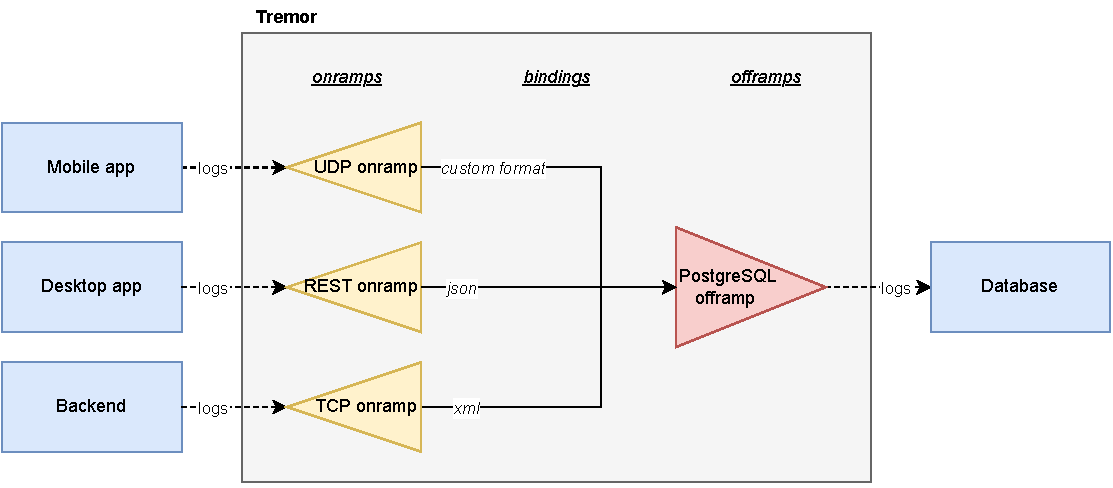
\includegraphics[width=\textwidth]{./Imagenes/example.pdf}
    \caption{Ejemplo de uso de Tremor}%
    \label{fig:example_tremor}
\end{figure}

\begin{figure}
    \centering
    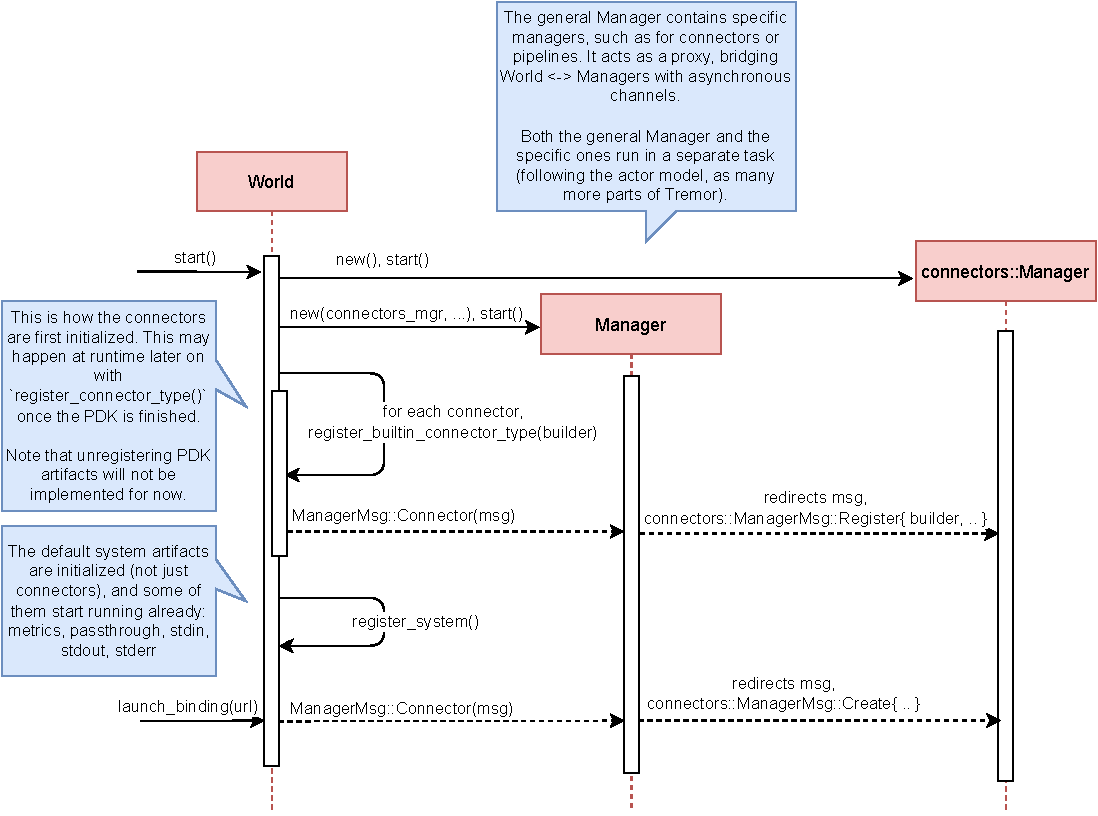
\includegraphics[width=\textwidth]{./Imagenes/registering.pdf}
    \caption{Ejemplo de uso de Tremor}%
    \label{fig:example_tremor}
\end{figure}

\begin{figure}
    \centering
    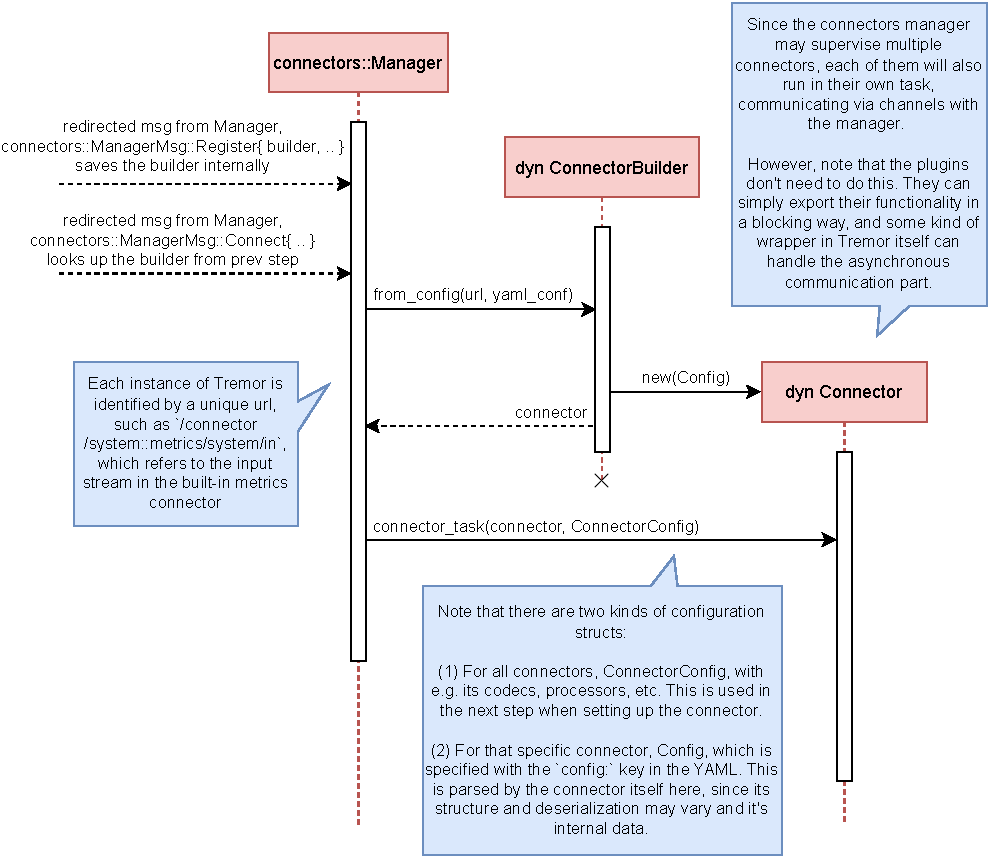
\includegraphics[width=\textwidth]{./Imagenes/initializing.pdf}
    \caption{Ejemplo de uso de Tremor}%
    \label{fig:example_tremor}
\end{figure}

\begin{figure}
    \centering
    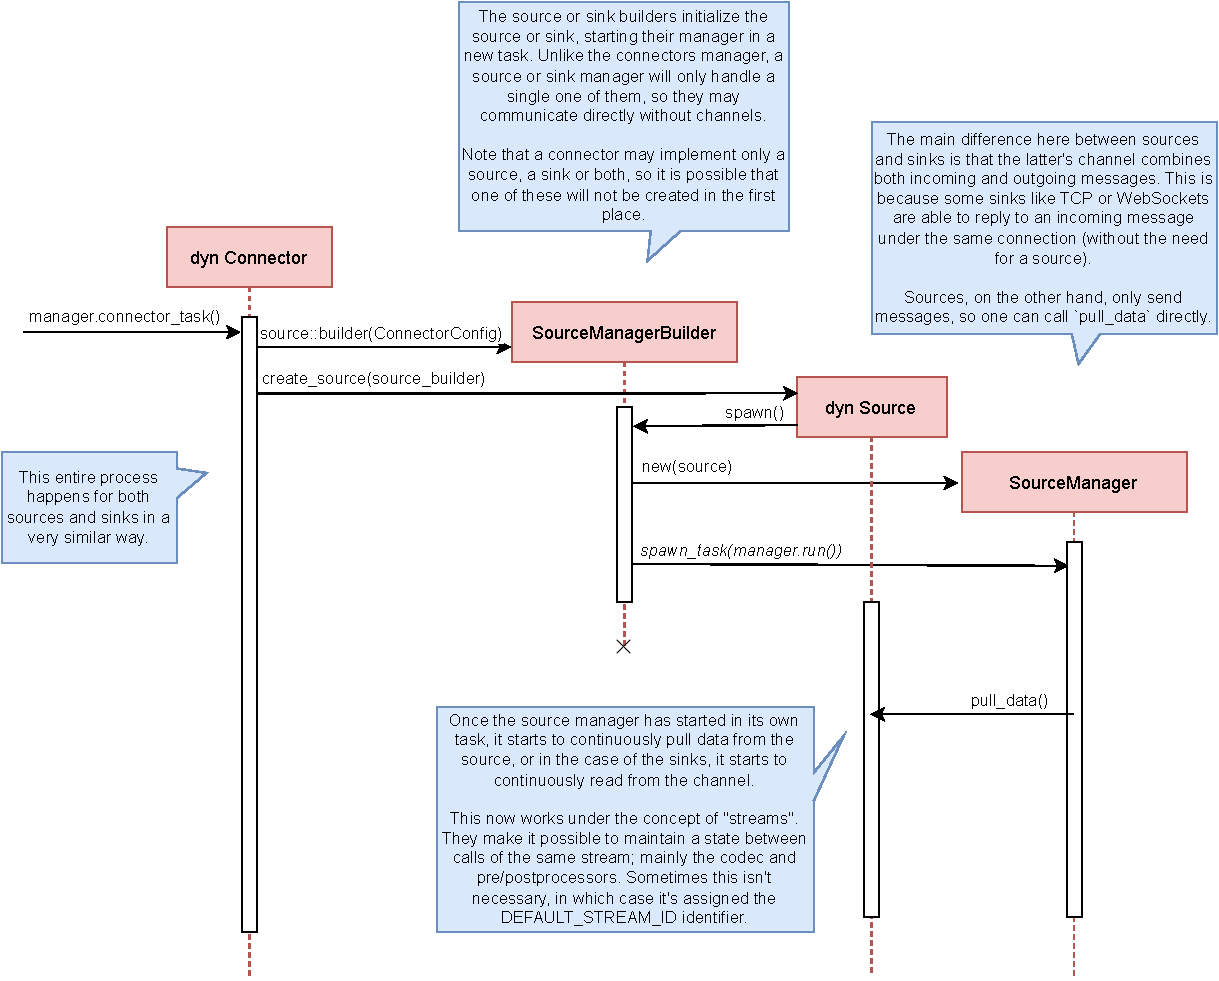
\includegraphics[width=\textwidth]{./Imagenes/setting-up.pdf}
    \caption{Ejemplo de uso de Tremor}%
    \label{fig:example_tremor}
\end{figure}
